% !TEX root = ../../report.tex
\clearpage
\section{Experimental Plan}
\label{sec:experimental-plan}

%We can sometimes evaluate how well the recommender achieves its overall goals.
%For example, we can check an e-commerce website revenue with and without the
%recommender system and thereby estimate the value of the system to the website.

This section will cover our experimental plan, starting off by looking at the
goals for our experiments, and how we plan on getting there. The remaining parts of
the section will describe the datasets used for evaluation, our evaluation methodology.
We have the following main goals for our experiment:

\begin{itemize}
	\item Determine the effect of utilizing multiple event types
	\item Determine whether our proposed implicit rating methods improve the recommendation quality over
	binary preference data.
	\item Evaluate the different implicit rating features and attempt to quantify their importance.
	\item Quantify the value of adding a cold-start solution method to the system.
	\item Propose a \emph{best} combination of methods, given our current limitations for the SoBazar recommender system.
\end{itemize}

As baselines for our project we wish to first test a set of binary methods on the SoBazaar data
looking only at \emph{purchases}. We do the same for a binary dataset including the events
\emph{purchase}, \emph{wants} and \emph{likes}. We then want to test our \emph{implicit ratings}
considering different factors such as \emph{implicit factor weighting}, \emph{global popularity},
\emph{recency} and factors blended together using different schemes and see if they improve the
recommendation quality.

\subsection{Comparing Ratings}

The success on our experiment mainly relies on whether we can successfully compare a set of ratings.
Evaluating and comparing a set of ratings is not something you often encounter in the literature. 

\begin{figure}[H]
		\centering
	  	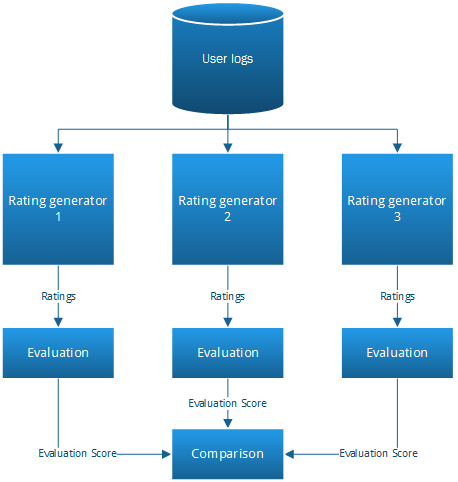
\includegraphics[scale=0.7]{image/ratinggeneval.png}
		\caption[Comparing Ratings]{The Figure shows the process of comparing ratings}
		\label{figure:compareratings}
\end{figure}

Our main challange is to come up with a reasonable evaluation function which could support
our hypotheses. The bottom line is that evaluating and comparing a set of ratings is hard.
However, we have a few theories on how it can be done:

\begin{enumerate}
\item Can we put the ratings into a traditional recommender system evaluation pipeline and use the
	  results from that to compare the ratings. In that case, what evaluation metrics are suitable?
\item User studies. Ask users to evaluate how well the produced ratings fit their actual preferences \cite{parra2011walk}.
\item Online experiments measuring e.g. the increased revenue generated or the click-through-rate of the recommendations.
\end{enumerate}

User studies are expensive and we simply do not have the time or resources to interview hundreds of actual users.
We do also not have the option of performing any online experiments. Either way it would be best to
get some kind of validation on our results before deploying the system to minimize the risk of giving
low-quality recommendations to the users.

We therefore \emph{chose} to go for the first alternative, despite it having a few obvious weaknesses.
Our main assumption is that better ratings give better recommendation recommendation results, and use this
as a basis for our evaluation. However, this means that the results we get from testing them
on different algorithms should be comparable. There are two main problems with this. The first is that
we rely on a recommender algorithm can make use of our implicit ratings. We also need to be careful
when selecting evaluation metrics. Many evaluation metrics consider supplied ratings as the \emph{ground truth}
and bases its evaluation score on these numbers. This automatically disqualifies any evaluation metrics
that consider the rating values such as e.g. MAE. After some thought and consideration
we identified the following properties as the best indicators of improved recommendation quality.

\begin{itemize}
\item Does it improve the recall?
\item Does it improve the recommenders ability to rank the items?
\end{itemize}

A further discussion on evaluation metrics will follow in the next Section \ref{sec:eval-metrics}.

\subsubsection{Purchase Only Vs. Multiple Implicit Factors}

We want to evaluate whether a recommender system utilizing multiple implicit factors is \emph{better}
a recommender system utilizing purchase data only. Firstly, we have two completely different datasets.
One containing multiple items and user not found in the other dataset. Secondly, one dataset
contains a set of ratings considered irrelevant by the other. This means that our comparison
\emph{must} be made on a subjective basis. However, we believe it safe to assume that recommending
a loved or clicked item is better than recommending no items at all. In addition we should also
factor in the added coverage.

\subsubsection{Comparing Binary and Non-Binary Models}

We want to quantify the improvements if any from using implicit ratings over binary ratings.
The main challenges of comparing the binary ratings with the non-binary ones are the fact
that the models for making recommendations differ. Optimally you would like to fix every
\emph{variable} when doing this comparison, however, it is not possible in this case.
To \emph{solve} this problem we decided that the best solution was to select \emph{state-of-the-art}
methods from both classes and compare their results. Worst case scenario we find out that the
methods for non-binary implicit feedback are not as \emph{good} as the binary models and thus
should not be used.

\subsubsection{Comparing Implicit Rating Methods}

We want to figure out how to evaluate and compare the different implicit rating
methods.  The most obvious solution here is to compare their recommendation performance. This is
mainly a evaluation metric problem. Which will be discussed at length in the
next Section \ref{sec:eval-metrics}.

\subsection{Combining Implicit Ratings With Existing Cold-Start Solutions}

%Only use cold-start splits for this sections tables.

After the best method have been chosen we wish to further improve our results
by adding a cold-start solution to our system. In the second stage of our
experiment we wish to see if we can apply a cold-start solution to increase the
systems cold-start performance. We therefore need to simulate the different cold-start
scenarios and measure the methods ability to deal with these scenarios.

\subsubsection{Dataset}

In addition to evaluate the methods on the SoBazaar dataset we want to make sure that our
methods generalizes beyond our experimental dataset, in accordance to the general guidelines
for experimental studies \cite{Shani2011}. The data used for offline evaluation should match
as closely as possible the data we expect the recommender system to face when it is
deployed \cite{Gunawardana2009}. When selecting datasets for evaluation we focused on the
following dataset properties:

\begin{itemize}
	\item Size of dataset: Preferable as close as possible to SoBazaar or larger (a few months from now)
	in terms of number of ratings, users and items.
	\item Different different types of implicit factors	such as clicks, likes and purchases.
	\item Domain: Preferably a domain as close to possible as the e-commerce domain where
	factors like recency also would apply.
	\item Timestamps: To evaluate the recentness mapping
	\item Presence of features (Secondary)
\end{itemize}

We were unable to acquire any e-commerce datasets containing user browsing history including different event types
and timestamps. Thus making the main contributions of this article untestable, thus rendering further experiments
on other datasets useless. It is worth nothing that we inquired other researchers having
experimented with similar datasets to no luck.

\paragraph{The SoBazaar Dataset}

The SoBazaar dataset is small and sparse dataset. When looking only at the purchases
we have a total of 1,592 binary ratings given by 466 users to 1188 items. When including
clicks, wants and purchases we end up with 27,873 ratings given by 1,511 users to 5,855 items.
We also have access to semi-structured product information collected/crawled from
the online retailers for \emph{a majority} items.

Having such a small and sparse dataset has several implications. Firstly we have
to avoid \emph{wishful thinking} as we have very thin data, meaning that we cannot
rely on getting reliable results. Secondly, our evaluation methodology must be
\emph{tailored} for small sparse datasets. E.g. when using cross-validation the number
of folds depends on the size of the dataset. For large datasets, even 3-fold Cross
validation will be quite accurate, while for very sparse datasets, one may have to
use leave-one-out in order to train on as many examples as possible. The advantages
of using a large number of folds is that the bias of the true error rate estimators
will be small, meaning that the estimator will be very accurate, with the disadvantages being that
the variance of the true error rate estimator will be large in addition to increased
computation time. Another alternative well suited for sparse datasets is the
\emph{all but one} or the \emph{leave one out} method, in which we remove one rating
from the test users and try to predict the hidden rating.

Another important concern is whether or not to take the timestamps into consideration,
which directly speaks against the use of cross-validation, as we wish to use the past
interactions to predict future actions. When using the \emph{leave one out} method one
could e.g. always remove the users freshest rating and try to predict it and repeat the
process any number of times. This is particularly relevant as some of our implicit mapping functions
factors in recency.

\subparagraph{Overview of the Dataset}

The following table shows an overview of the purchase only and multiple event SoBazaar datasets:


\begin{table}[H]
    \centering
    \begin{tabular}{l l l l l l }
    \toprule
	Dataset						& 	Ratings		& 	Users		& 	Items 		& 	Sparsity			& Rating Scale 				    \\ \midrule
	Sobazar	(Purchases Only) 	&	1,592		&	466			&	1188		&	99.71243			& Binary						\\
	Sobazar (All events)		& 	27,873  	& 	1,511		&	5855		& 	99.69657			& Binary/Implicit Ratings		\\
	%Movielens 1M				& 	1,000,029   &	6040 		&	3706		&	95.53164			& Explicit (1-5)				\\
	\bottomrule
    \end{tabular}
    \caption [Overview of the datasets used for evaluation]{Overview of the datasets used for evaluation}
    \label{table:datasets}
\end{table}

As you can see the recommender can cover a much larger portion of the user group and items when including multiple event types. However,
the sparsity is only reduced slightly as the number of items and users are much higher.

\subsubsection{Simulating the Cold-Start Problem}

To simulate the cold-start problem and evaluate how well our the different
methods tackle the different cold-start situations we use the following
evaluation methodology. As mentioned in Section \ref{sec:cold-start-eval} there
is no common framework for assessing the cold-start performance of recommender
systems.  Our goal is to come up with \emph{comprehensive} framework to assess
the cold-start performance of our recommender systems. The following inputs
changes the dataset over time:

\begin{itemize}
	\item 	Existing users watch new items in the catalogue
	\item	New users join the system and view their first item
	\item	New items are added to the catalogue
\end{itemize}

The first input source has the effect of increasing the dataset density, the
average user profile length, and the average number of views per item. The
second input factor has the effect of decreasing both the dataset density and
the average user profile length, as the new users that join the system have
interacted with only a few items. Similarly, the third input factor has the
effect of decreasing both the dataset density and the average number of views
per item.

To simulate the cold-start user problem we propose splitting the users into two
disjoint sets, similarly as in \cite{Stern2009, Lam2008}, using 90\% of the
users for training and setting aside the remaining 10\% for evaluation. We then
train the model with 10\%, 40\% and 75\% of the test users ratings and evaluate
the predictions for all models. The implications of removing the top 10\% of the raters from the
Sobazar dataset is fairly large as they stand for a large portion of the total ratings.
Similarly, to simulate the cold-start item problem we again split the items into two
disjoint sets, using 95\% of the items for training and the remaining 5\% for
evaluation. The reason for only using 5\% of the items is due to the low number of
ratings for most items. All test items must have been rated by at least 15 users.
We then train the model using 10\%, 40\% and 75\% ratings and predict the remaining values. The
selection criteria for test items and users can differ from dataset to dataset.
E.g. in \cite{Rashid2002, Rashid2008} the authors selected a subset of the
users with more than 200 ratings, but you can not expect 10\% all the users for
all datasets to have provided 200 ratings, so this number might be lowered if
necessary, as in our case. To evaluate the cold-start system performance we use the same method as
described in ~\cite{Agarwal2009}. We use a 80:20 training/test split, where
we at random draw 40\%, 60\% and 80\% (all) ratings and predict the 
remaining 20\% for all models. It is important to note that this process should be repeated multiple times, as
the chance of getting an \emph{unfortunate} split is highly probable due to the
dataset size. We perform both random and time-based splits. For our time based
splits we train the model with e.g. 10\% of the first ratings given by the
user and try to predict the remaining 90\%. Similarly for the cold-start
system splits we train the model using a random subset of the 80\%
earliest ratings and try to predict the remaining 20\%.
